\colorbox{green}{TEMPORARY - CM8}

However, this approach converges quite slowly: the accuracy, measured by the standard deviation, is $\sim \frac{1}{\sqrt{n}}$. We would need a lot of needles...

\subsection[Another way to compute  \texorpdfstring{$\pi$}{pi}]{Another way to compute $\pi$}

Let us first notice that $\pi$ is simply the area of a unit disc. Thus $\frac{\pi}{4}$ is the area under the red curve of figure~\ref{fig:quart_disc}. Then a new random algorithm to compute $\pi$ is simply:
\begin{itemize}
	\item Pick $n$ random points $(x,y)$ uniformly in $[0,1]^2$;
	\item Define $k:=|\{(x_i,y_i):x_i^2+y_i^2<1\}|$;
	\item $\frac{\pi}{4}\approx \frac{k}{n}$
\end{itemize}

This algorithm is very similar to the one using the needles, instead that this one can easily be implemented on a computer. Therefore the analysis of convergence remains the same: the accuracy evolve like $\sim \frac{1}{\sqrt{n}}$ (slow convergence).

\begin{figure}[h!]%height=0.3\linewidth ,
    \centering
    \subfloat[$\frac{\pi}{4}=$ area under the red curve.]{\label{fig:quart_disc}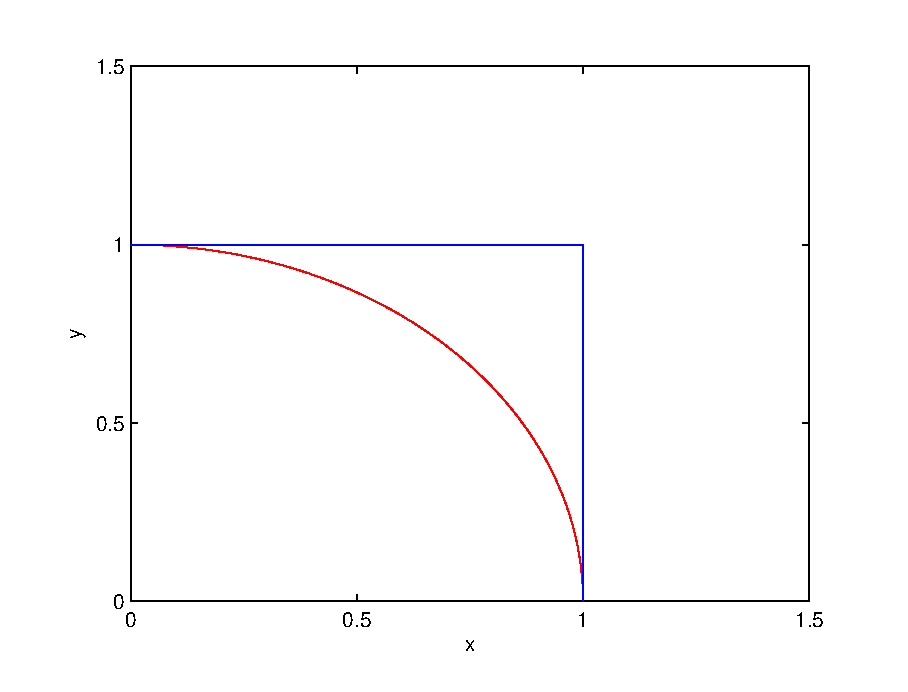
\includegraphics[width=0.5\linewidth ]{./images/figure_quart_disc.eps}}~
		\subfloat[]{\label{fig:quart_disc_xi}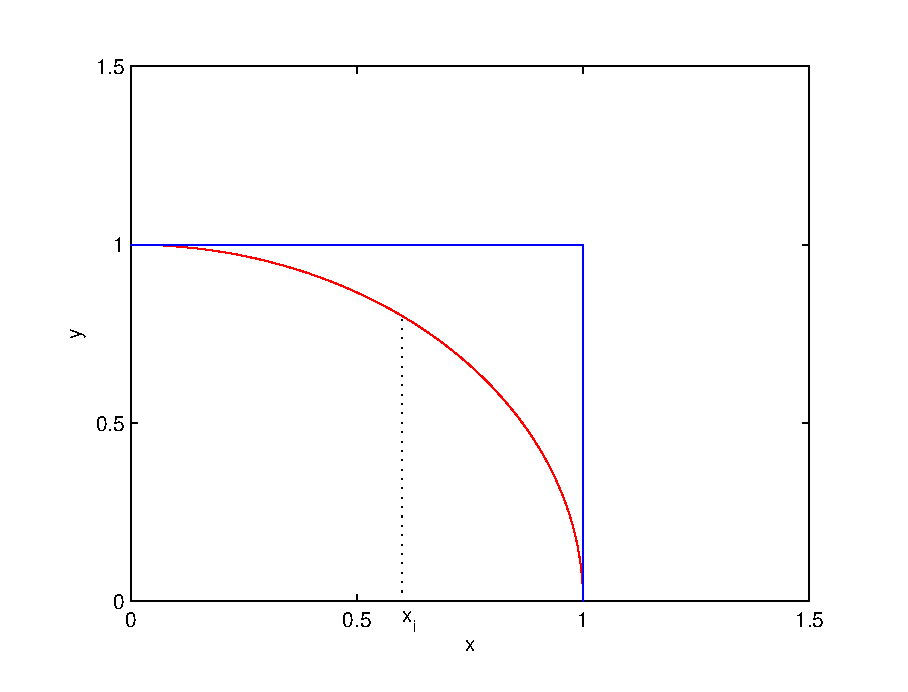
\includegraphics[width=0.5\linewidth ]{./images/figure_quart_disc_xi.eps}}\\
		\caption{} 
		\label{fig:compute_pi}
\end{figure}

\subsection{A bit smarter}

We can easily improve the last naive $\pi$ estimation:
\begin{itemize}
	\item Pick $x_i$ randomly between $0$ and $1$ (see figure~\ref{fig:quart_disc_xi});
	\item Compute\footnote{For a fixed $x_i$, the probability for the associated $y_i$ to be such that $(x_i,y_i)$ lies under the red curve of figure~\ref{fig:quart_disc_xi}, is $\frac{\sqrt{1-x_i^2}}{1}$, under uniform distribution. Since we know this probability, we can use it directly instead of picking a random $y_i$!}
\[
	\begin{array}{ll}
	\frac{\sum_{i=1}^n{\sqrt{1-x_i^2}}}{n}&\approx \E\left[\sqrt{1-x^2}\right] \text{  under uniform distribution of }x\\
	&:=\int_{0}^1{\sqrt{1-x^2} dx} \text{  by definition of } \E\\
	&=\frac{\pi}{4}
	\end{array}
\]
\end{itemize}

Again the error of this algorithm decreases like $\sim \frac{1}{\sqrt{n}}$.\\

This method generalizes into a random computation of integrals. 1D integrals are usually better evaluated by deterministic methods (rectangles, simpson, ...). Indeed, the error of the rectangles method (the simplest deterministic method) is in $\frac{1}{n}$, far better than $\frac{1}{\sqrt{n}}$.

\section{Why use this random algorithm for integration?}
For at least two reasons:
\begin{description}
\item[Robin hood effect: ] For every deterministic method, there are functions for which the method will fail. For example, for high frequency sine (see figure~\ref{fig:high_freq_sine}), if the red points are chosen as equally spaced quadrature points, the deterministic method will give a very poor estimate of the integral.\\

Thus deterministic methods have very bad worst case behaviour. The choice of random points makes all instances "equal".
\item[For kD integrals: ] $\underbrace{\int \int \hdots \int}_{k} f(x_1,\hdots,x_k)dx_1\hdots dx_{k}$

For deterministic methods, $n$ points regularly spaced in $[0,1]^k$ $\rightarrow \sqrt[k]{n}$ points in each dimension (see figure~\ref{fig:kD_int}: by choosing the 4 red points, we have 2 blue points in each dimension). Typically, the error will be $\sim \frac{1}{\sqrt[k]{n}}$ (when $k$ increases, we need more points to fill the space\footnote{Thus with fixed $n$, we have less information along each dimension and thus the accuracy decreases.}).\\

The random algorithm still behaves in $\frac{1}{\sqrt{n}}$ error (because it depends on the properties of the gaussian distribution) and could possibly be a better choice for triple integrals or more (a hybrid method is even better).
\end{description}

\begin{figure}[h!]%height=0.3\linewidth ,
    \centering
    \subfloat[High frequency sine.]{\label{fig:high_freq_sine}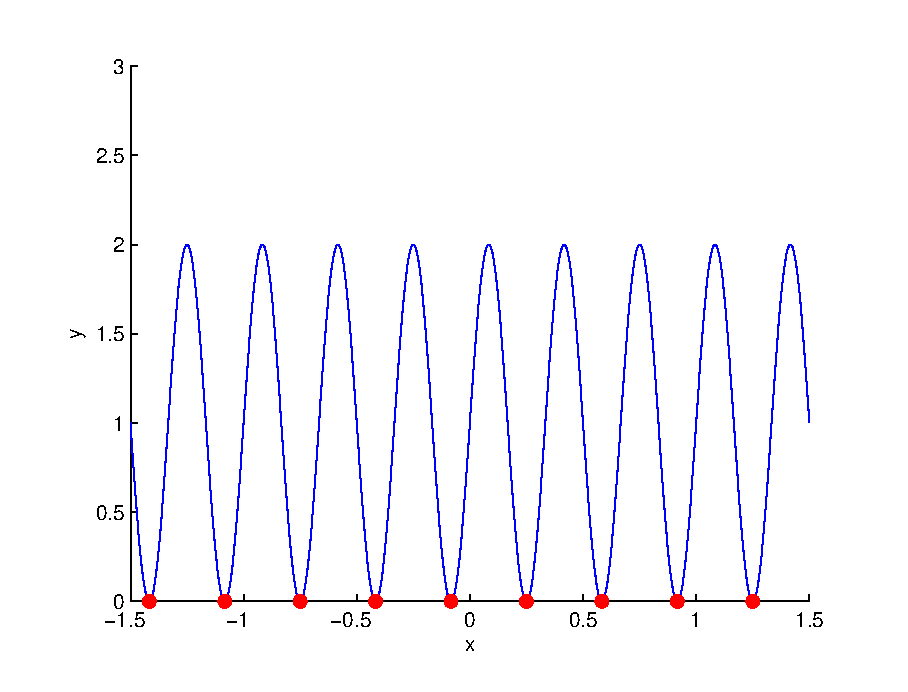
\includegraphics[width=0.5\linewidth ]{./images/high_freq_sine.eps}}~
		\subfloat[]{\label{fig:kD_int}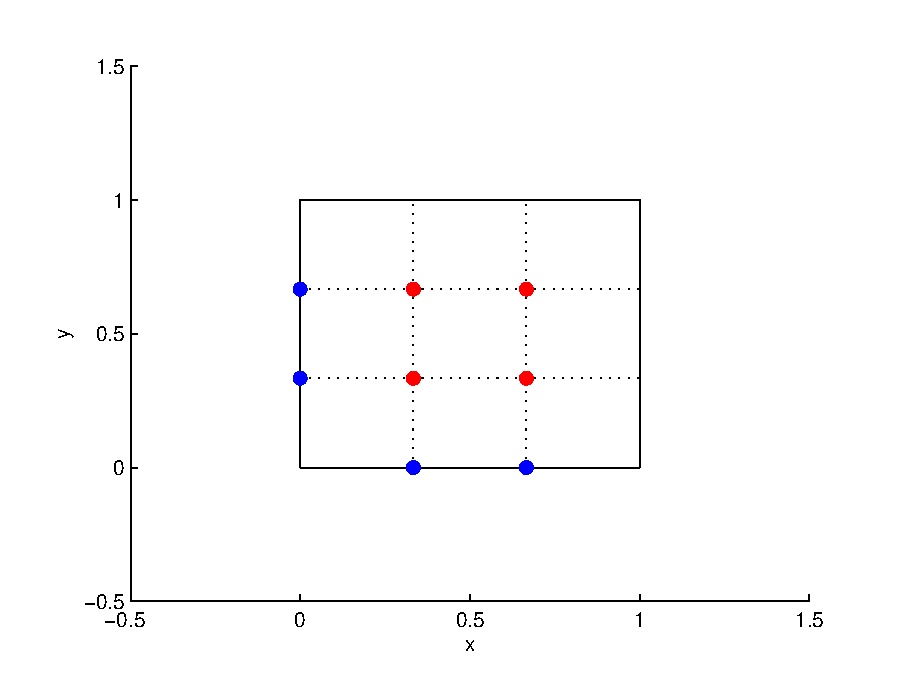
\includegraphics[width=0.5\linewidth ]{./images/kD_int.eps}}\\
		\caption{} 
		\label{fig:R_A_integration}
\end{figure}

\section{Monte-Carlo Algorithms}
\subsection{An example where randomness is very useful}

Suppose you want to check that $A\cdot B=C$, with $A$, $B$ and $C$ $n\times n$ matrices.
\begin{itemize}
	\item Obvious method: compute $A\cdot B$. It costs $\mathcal{O}(n^{2,3\hdots})$ (using divide and conquer methods). If $n$ is large, then this method might take a lot of time.
	\item Compute $\left( A\cdot B\right)_{i,j}$ ($\mathcal{O}(n)$ time) and compare with $C_{i,j}$ for random $i$, $j$. However if there is only one wrong $C_{i,j}$, it is hard to capture it using this method. We would like a method which finds errors with good probability, even if they are really localized.
	\item If $A\cdot B=C$ then $\forall v\in \R^{n\times 1}$, $\underbrace{A\cdot B\cdot v}_{\mathcal{O}(n^2)}=\underbrace{C\cdot v}_{\mathcal{O}(n^2)}$ (this solution is not localized but spread on the columns, by checking if $A\cdot B=C$ in the direction of $v$). How to pick $v$? Randomly in $\{0,1\}^n\rightarrow$ summing a subset of columns of $A\cdot B$ (resp. $C$) $\Rightarrow A\cdot B \cdot v$ (resp. $C\cdot v$).\\
\end{itemize}

	Say there is an error in column $j$ of $C$ (and possibly elsewhere). $\forall v\in \{0,1\}^n$, call $v_{\bar{j}}=v$ except that entry $j$ is flipped ($0 \leftrightarrow 1$). 
	\begin{itemize}
		\item Either $A\cdot B\cdot v\neq C\cdot v$ and $A\cdot B\cdot v_{\bar{j}}\neq C\cdot v_{\bar{j}}$;
		\item or $A\cdot B\cdot v= C\cdot v$ and $A\cdot B\cdot v_{\bar{j}}\neq C\cdot v_{\bar{j}}$;
		\item or $A\cdot B\cdot v\neq C\cdot v$ and $A\cdot B\cdot v_{\bar{j}}= C\cdot v_{\bar{j}}$;
		\item but $A\cdot B\cdot v= C\cdot v$ and $A\cdot B\cdot v_{\bar{j}}= C\cdot v_{\bar{j}}$ is impossible because then 
		$$\underbrace{A\cdot B \cdot (v-v_{\bar{j}})}_{\pm j^{th} \text{ column of } A\cdot B}=\underbrace{C\cdot (v-v_{\bar{j}})}_{\pm j^{th} \text{ column of } A\cdot B}$$
		which is impossible since there is a mistake in $j^{th}$ column of $C$!
	\end{itemize}
	Therefore at least half of possible $v\in \{0,1\}^n$ will show an error $\Rightarrow$ Error detected with probability $\geq \frac{1}{2}$ (if there is at least one error).\\
	
	This leads us to Freivalds algorithm:
	\begin{lstlisting}[caption={Freivalds Algorithm ($A$,$B$,$C$)}]
	Pick  v in {0,1}^n randomly (using uniform distribution);
	If A*B*v==C*v
		then print "A*B=C" [maybe];
	Else A*B*v~=C*v 
		then print "A*B~=C" [for sure].
	\end{lstlisting}
	
	However with this algorithm, false negatives (i.e. $A\cdot B\neq C$ but undected, with probability $\leq \frac{1}{2}$) are possible... To improve Freivalds, we can use amplification of stochastic advantage\footnote{We can try again with other $v$! We will never be sure that $A\cdot B=C$, but the probability of error will decrease a lot if we test a lot of $v$.}:
	\begin{lstlisting}[caption={Repeat($A$,$B$,$C$,$k$)}]
		Repeat Freivalds k times;
		If k conclusions "A*B==C" 
			then print "A*B=C" [maybe];
		Elseif at least one conclusion "A*B~=C" 
			then print "A*B~=C" [for sure].
	\end{lstlisting}
	A mistake will go undetected with probability $\leq \frac{1}{2^k}$. For example, with $k=10\Rightarrow \frac{1}{2^k}\approx 10^{-3}=0.1\%$, with time $\mathcal{O}(kn^{2})$ which is better than $\mathcal{O}(n^{2,3...})$ or $\mathcal{O}(n^{3})$.\\

	%This is a nice property of stochastic algorithms: by repeating them, we can improve their conclusions. 
	Amplification of stochastic advantage is very powerful when errors on a decision problem (YES/NO problem\footnote{Answer to the problem is binary; $\neq$ compute $\pi$.}) are one-sided: $\exists$ false negative, $\nexists$ false positives, or the contrary (in our case, if we print "$A\cdot B\neq C$", it is for sure).\\

\subsection{Monte-Carlo Algorithms}

	What now if you get possible false negatives and false positives (for other problems)? E.g.:
	\begin{itemize}
		\item answer is YES but we conclude YES with probability $\geq \frac{1}{2}+\epsilon$;
		\item answer is NO but we conclude NO with probability $\geq \frac{1}{2}+\epsilon$;
	\end{itemize}
	(the algorithm gives us slightly more often the good answer that when we throw a coin)
	
	Amplification of stochastic advantage still works!

  Repeat $n$ times and vote among the answers:
	\begin{itemize}
		\item If $>50\%$ of YES $\Rightarrow$ output YES;
		\item if $>50\%$ of NO $\Rightarrow$ output NO.
	\end{itemize}
	What is the probability of error? We can use indicator variables. Let
	$$X_i=\left\{
	\begin{array}{ll}
       1&\text{if }i^{th}\text{ run is correct}\\
       0&\text{if }i^{th}\text{ run is wrong}
%\mbox{sinon}
			\end{array}
  \right.
  $$
	Then we have $\E[X_i]\geq \frac{1}{2}+\epsilon$. Let us say that $\E[X_i]=\frac{1}{2}+\epsilon$, to study the worst case.
	
	The repeated algorithm is wrong if $\sum_{i=1}{X_i}<\frac{n}{2}$. But 
	\begin{align*}
	\E\left[\sum_{i=1}^n{X_i}\right]&=\left(\frac{1}{2}+\epsilon\right)n\\
	\mathrm{Var}\left[X_i\right] &= \E\left[X_i^2\right] - \left(\E[X_i]\right)^2\\
	&=1\cdot \left(\frac{1}{2}+\epsilon\right)+0\cdot \left(\frac{1}{2}-\epsilon\right) - \left(\frac{1}{2}+\epsilon\right)^2\\
	&=\frac{1}{4}-\epsilon^2\\
	\mathrm{Var}\left[\sum_{i=1}^n{X_i}\right]&=n\cdot \left(\frac{1}{4}-\epsilon^2\right)\text{ using independence of }X_i\text{'s}
	\end{align*} 
	Using the Central Limit Theorem, $\sum_{i=1}^n{X_i}\sim \text{Gaussian}\left( \left(\frac{1}{2}+\epsilon\right)n,\left(\frac{1}{4}-\epsilon^2\right)n \right)$ if $n$ is large. Using the tables, $\sum_{i=1}^n{X_i}$ has $2.5\%$ of probability to be 2 standard deviations above its mean.
	
	E.g. $\epsilon \cdot n=2\cdot \text{ (standard deviation)}=2\sqrt{n}\sqrt{\frac{1}{4}-\epsilon^2} \Rightarrow n=\frac{4}{\epsilon^2}\left(\frac{1}{4}-\epsilon^2\right)\sim \frac{1}{\epsilon^2}$ for small $\epsilon$. Then we have the wrong answer with probability $\leq 2.5\%$.
	
	If $\epsilon\cdot n=3\cdot (\text{standard deviation})\Rightarrow n\sim \frac{9}{4\epsilon^2}$, then we get the wrong answer with probability $\leq 0.15\%$.
	
	Thus amplification of stochastic still works, but we need to perform more trials then when only false negatives (or false positive) are appearing. Also we can notice that if $n\sim \frac{1}{\epsilon^2}$ is approximately doubled (so that $n\sim \frac{9}{4\cdot \epsilon^2}$), the probability of error decreases much.\\
	
	These algorithms provide an uncertain answer (correct with some probability). They are called Monte-Carlo algorithms (they provide possibly wrong answer):
	\begin{itemize}
		\item estimate $\pi$;
		\item estimate $kD$ integrals;
		\item Freivalds;
		\item checking that a number is prime (like Freivalds, error is one-sided);
		\item generating a large prime number\footnote{The last two items are useful in cryptography.}.
	\end{itemize}
\vspace{0.5cm}

\section{Las Vegas Algorithms - Eight Queens problem}
Another sort of algorithms are those that provide a correct answer always, but with random execution time. They are called Las Vegas algorithm. E.g., Random QuickSort, Random selection/Median, ...

Let us see a Las Vegas algorithm for the Eight Queens problem: how to place 8 queens in a chessboard in mutually non-attacking positions, i.e.
\begin{itemize}
	\item no two queens in the same row;
	\item no two queens in the same column;
	\item no two queens in the same diagonal;
\end{itemize}

\subsection{Brute force solution}
Explore systematically the tree of possibilities, \textbf{backtracking} when you reach a dead-end:
\begin{itemize}
	\item place a queen on the first row;
	\item place a queen on the second row (but different column);
	\item place a queen on the third row (but different column);
	\item $\vdots$
	\item avoiding same diagonal-positions.
\end{itemize}
\subsection{The random 8 queens algorithm makes random choices}
\begin{itemize}
	\item random column for the $1^{st}$ queen (in $1^{st}$ row);
	\item random column for the $2^{nd}$ queen (but $\neq$ from the first one and among the valid squares for diagonals)
	\item ...
\end{itemize}
If there is no more solution to place a new queen, we repeat \textbf{from scratch} $=$ no memory of previous attempt (it is the difference with the backtracking solution). We can compute that 

% \underbrace{....}_{\substack{\text{Some long text that}\\\text{should be multiline}}}


\begin{align*}
\E\left[ \text{time success}\right]&=\underbrace{\text{Time}_{\text{in case of Success}}}_{\substack{\text{time to fill in the chessboard }\\\text{ for the final solution}}} + \left[\frac{1}{P[Success]}-1\right]\cdot \text{ Time}_{\text{in case of failure}}
\end{align*}
\begin{align*}
\text{because } \frac{1}{P\left[success\right]}&=\E\left[\text{number of runs to get a success}\right]=\E\left[\text{number of failure}\right]
\end{align*}


Thus we have \footnote{The 6 in the equation comes from the fact that on average we have 5 or 6 queen placement in a failure}
\begin{align*}
\E\left([\text{time success}\right]&=8+(\frac{1}{0,129...}-1)\cdot 6 \text{ queen placements}\\
&\approx 50\text{ or }60\text{ queen placements}
\end{align*}

whereas the backtracking solution will get a success after 155 queen placements.\\

Furthermore the gap grows quickly when 8 queens $\Rightarrow n$ queens (when we increase the number of queens to place). This is at first sight surprising because the random algorithm and the backtracking solution explore the same possibilities but in different orders.\\

The random algorithm needs less time because placements have nothing "regular".